\documentclass[11p]{article}
% Packages
\usepackage{amsmath}
\usepackage{graphicx}
\usepackage{fancyheadings}
\usepackage[swedish, english]{babel}
\usepackage[
    backend=biber,
    style=authoryear-ibid,
    sorting=ynt
]{biblatex}
\usepackage[utf8]{inputenc}
\usepackage[T1]{fontenc}
\usepackage{titlesec}
\usepackage{hyperref}
%Källor
\addbibresource{references.bib}
\graphicspath{ {./images/} }

% Lite variabler
\def\email{levi.hogdal@elev.ga.ntig.se}
\def\foottitle{Gymnasiearbete} % Kanske borde ändras
\def\name{Levi Högdal}

\title{Gymnasiearbete \\ \small Gymnasiearbete}
\author{\name}
\date{\today}


\begin{document}



% fixar sidfot
    \lfoot{\footnotesize{\name \\ \email}}
    \rfoot{\footnotesize{\today}}
    \lhead{\sc\footnotesize\foottitle}
    \rhead{\nouppercase{\sc\footnotesize\leftmark}}
    \pagestyle{fancy}
    \renewcommand{\headrulewidth}{0.2pt}
    \renewcommand{\footrulewidth}{0.2pt}

% i Sverige har vi normalt inget indrag vid nytt stycke
    \setlength{\parindent}{0pt}
% men däremot lite mellanrum
    \setlength{\parskip}{10pt}
    \begin{otherlanguage}{swedish}


        \begin{titlepage}
            \centering

            % Title and subtitle are enclosed between two rules.
            \rule{\textwidth}{1pt}

            % Title
            \vspace{.7\baselineskip}
            {\huge \textbf{Tillgänglighet på Sveriges kommuners webbplatser}}

            % Subtitle
            \vspace*{.5cm}
            {\LARGE Webbplatserna anpassning till WCAG 2.2 standarden och generellt användarvänlighet}

            \rule{\textwidth}{1pt}

            \vspace{1cm}

            % Set this size for the remaining titlepage.
            \large

            % Authors side by side, using two minipages as a trick.
            \begin{minipage}{.5\textwidth}
                \centering
                \name \\
                {\normalsize \url{levihogdal@elev.ga.ntig.se}}
            \end{minipage}%

            \vspace{3cm}

            % Report logo.
            
\includegraphics[width=0.4\textwidth]{../images/NTI Gymnasiet_Symbol_print_svart.png}

            \vfill

            % University and date information at the bottom of the titlepage.
            NTI Gymnasiet Umeå \\
            Teknikprogrammet\\
            Gymnasiearbete\\
            Datum: \today \\
            Handledare: Jens Andreasson
        \end{titlepage}
    %\maketitle
    %\begin{center}
    %
\includegraphics[width=0.4\textwidth]{../images/NTI Gymnasiet_Symbol_print_svart.png}
    %\end{center}
    \end{otherlanguage}


    \newpage
    \begin{otherlanguage}{english}
    \begin{abstract}
        Accessibility on the internet is important for the user and the creator of a website.
        All users should be able to use and understan a website if they understand the language of the website.
        This study aims to test the accessibility guidelines WCAG 2.2 on the websites of Swedish municipalities (kommuner).
        The study also includes if municipalities with less population meet less of the WCAG 2.2 criteria.
        %Because municipalities in general were tested the study also includes if municipalities with less population meet less of the WCAG 2.2 criteria.
        The method to accomplish this was to test each criteria of WCAG on all the chosen websites.
        %How each criteria of WCAG 2.2 was tested and the results were combined in a spreadsheet that can be found at the end of the study.
        None of the websites meet all the tested WCAG criteria. %fråga jens
        The worst performing website met 47/70 of the tested criteria and the best performing website met 63/70 of the tested criteria.
        The study also showed that there might be a tendency for municipalities with less population to have a worse performing website but to draw such a conclusion more websites would have to be tested.

    \end{abstract}
    \end{otherlanguage}
    \begin{otherlanguage}{swedish}
    \newpage
    \tableofcontents
    \newpage

    \section{Inledning} %byt från hemsidor till webbplatser
    Att kunna använda och navigera en webbplats är något många nuförtiden tar för givet.
    Att förstå internet och kunna enkelt läsa och navigera olika webbplatser är inte det lättaste.
    Det finns många olika sätt som en webbplats kan se ut men hur ska webbplatser anpassas så att användare enkelt ta del av informationen.
    Om användaren inte är van med att använda webbplatser kan det bli väldigt svår att använda och tolka webbplatsen.
    För att användare ska kunna enklare förstå och använda flera olika webbplatser görs olika webbstandarder.
    Webbstandarden som den här undersökningen utgår ifrån är WCAG com är skapad av W3C.
    %För att underlätta utvecklingen av användarvänliga webbplatser har en organisation som heter W3C skapat standarder(WCAG) för användarvänlighet och tillgänglighet.

    
    \subsection{Syfte och frågeställning}
    Hur mycket webbplatser förhåller sig till WCAG standarden är varierande men studien är intresserad av hur olika kommunala webbplatser förhåller sig till dem och vilka olika delar av WCAG 2.2 standarden de möter.
    \\Det som ska undersökas är:
    \begin{itemize}
        \item Vilka WCAG 2.2 krav uppfyller kommuners webbsidor och vilka skillnader finns det i kraven som kommunerna uppfyller.
        \item Finns det några skillnader på antalet invånare i kommunen och hur många krav kommunen uppfyller.
    \end{itemize}

    \section{Bakgrund}

    \subsection{Tillgänglighet}
    Tillgänglighet i det här sammanhanget betyder inte hur åtkomligt webbplatsen är utom att den ska vara användbar för alla användare. %alla användare inkluderar dom med funktionsnedsättnig
    Tillgänglighet handlar om hur enkelt användaren kan förstå webbplatsen \parencite{webbriktlinjer}.
    I tillgänglighet på webben ingår väldigt mycket men för att ge några exempel ingår bland annat:
    Hur bra kontrast det är mellan bakgrund och text så att det ska vara enkelt att läsa texten.
    Blinkar webbplatsen för mycket så den är obehaglig att kolla på.
    Har ljudbaserad media textalternativ så om användaren är till exempel döve eller är i en högljudd miljö kan fortfarande ta del av informationen.
    \\Webbsidors design och utformning ska vara anpassad så att alla människor ska kunna använda och förstå webbsidan så länge de kan läsa språket.
    För att webbsidor ska vara tillgänglighets anpassade gör standarder som kan följas när webbsidor skapas och olika lagar.
    Webbstandarden som den här undersökningen utgår från är WCAG som är utgivet av W3C. %fråga jens


    \subsection{Webbsidors uppbyggnad}
    Webbsidor är nästan alltid uppbyggda i grunden av 4 olika delar: %fråga jens
    \begin{itemize}
        \item Hypertext markup language (HTML)
        \item Cascading style sheets (CSS)
        \item Accessible rich internet applications (ARIA)
        \item Javascript/Typescript (JS/TS)
    \end{itemize}
    Den här undersökningen är intresserad i HTML, CSS och ARIA men inte Javascript/Typescript.
    Javascript och Typescript är inte relevant till den här undersökningen.
    Javascript och Typescript används av själva servern för att hantera webbsidan men är inte något som klienten (användaren) interagerar med. %fråga jens

    \subsubsection{Hypertext markup language}
    % Du har feedback. Skriv om. %
    HTML är standardspråket som webbplatser skapas med.
    HTML är språket som ger struktur och definierar grunden till hur webbplatser ser ut \parencite{HTML}.
    Språket bestar av element som är skriven på följande vis <html> och </html>.
    Text skriven utanför ett element förlorar all semantisk mening och kommer att skrivas ut på webbplatsen som normal text.
    Om den istället skrivs mellan början och slutet av ett element kommer texten att bli påverkad av elementets funktioner och stilar.
    Det gör att texten automatiskt formateras efter elementet och att webbsidan kan förstå innehållet.
    Elementen kan ha tillägg som kallas attribut.
    Det kan till exempel vara ett id så att css och js kan hitta och interagera med specifikt det elementet och inte alla element av den typen.

    %Text som inte är i en tagg kommer att hanteras som normalt textinnehåll och skrivas upp på hemsidan som normal text.
    %Om texten skrivs mellan en öppnings tag och stängnings tagg kommer texten bli påverkan av elementets funktioner och stilar.
    %Den första <body> kallas för en öppnings tagg och är början av elementet och den andra </body> kallas för stängnings tagg och är slutet av elementet.
    %Man kan också skriva mer i en tagg till exempel <article id="article"> där det första ordet är vilket element det är och den andra i det här fallet är ett id som kan användas för att hitta och interagera elementet med exempelvis javascript.
    %En stängnings tag är alltid på följande vis: </p>, </body>, </main>, </head>, </div> och så vidare.

    \subsubsection{Cascading style sheets}
    CSS är ett språk som används för att bestämma hur en webbplats ser ut \parencite{CSS}.
    Grundstilarna i HTML gör en webbplats som fungerar men den kommer inte nödvändigtvis se ut som utgivaren av sidan vill eller vara tillgänglighetsanpassad.
    För att justera hur en webbplatsen ser ut och bestämma webbplatsens design används CSS.

    \subsubsection{Accessible rich internet applications}
    ARIA är extra roller och attribut till element som används för att göra en webbplats mer tillgänglig.
    ARIA har mest funktionalitet om webbplatsen navigeras utan mus och tangentbord. \parencite{ARIA}.
    Att implementera ARIA på ett felaktigt sätt gör en webbplats som är mindre användarvänlig så HTML element och attribut bör användas istället om det uppfyller samma funktion.
    
    \subsection{The world wide web consortium}
    The world wide web consortium (W3C) är det företaget som är utgivarna WCAG 2.2 standarden \parencite{W3C}.
    W3C är ett företag som grundades av Tim Berners-Lee med syftet att säkerställa webbens utveckling och framtid.
    För att uppnå målet har de skapat standarder för webben och har diskussioner med flera grupper och organisationer om webben.
    WCAG standarden har de skapat och det är den som undersökningen kommer att utgå ifrån.

    \subsection{Web content accessibility guidelines} %kolla hur wcag förklarar det här, kanske ändra namn
    Web content accessibility guidelines (WCAG) är en lista av riktlinjer för webben \parencite{WCAG_2.2}.
    Målet med riktlinjerna är att göra webben mer tillgänglig och användarvänlig så att alla användare kan enklare förstå och navigera webbplatsen.
    En del av WCAG standarden är att alla individuella krav ska kunna testas separat.
    De finns 3 olika nivåer av användarvänlighet i WCAG standarden.
    Det är level A, level AA och level AAA.
    Level A är nivån för grundläggande användarvänlighet.
    Level AA är stark användarvänlighet och brukar ses som målet för företag att nå. %utväckla
    Level AAA är fantastisk användarvänlighet.
    Den här nivån är inte alltid realistisk för en webbplatsen att nå. %utväckla
    WCAG 2.2 är den senaste versionen av WCAG när undersökningen gjordes och den är indelad i 4 stora kategorier.
    \\De olika delarna är:
    \begin{enumerate}
        \item Synlighet %Uppfattningsbar och synlighet?
        \item Manövrerbar
        \item Begriplighet
        \item Robust
    \end{enumerate}

    %Synlighet handlar om att information och innehåll ska vara synligt och tillgängligt för användare.
    \subsubsection{Synlighet} %Att läsa det här är pain and suffering. Typ för lite text i stycket. För mycket information.
    Synlighet handlar om att information och innehåll ska presenteras så att användaren kan ta del av innehållet.
    Kategorin innehåller bland annat att all information som inte är textbaserad ska det finnas ett textalternativ.
    Det ska finnas alternativ till tidsbaserad media, till exempel att videor har undertexter.
    Användaren ska kunna skilja på innehållet på webbplatsen, till exempel att skilja navigationen frå annat textinnehåll.
    %Synlighet är indelad i 4 underkategorier:
    %\begin{enumerate}
    %    \item All information som inte är textbaserad ska det finnas ett textalternativ.
    %    \item Det ska finnas alternativ till tidsbaserad media, till exempel att videor har undertexter.
    %    \item Program ska kunna förstå och tolka sidans innehåll.
    %    \item Användaren ska kunna skilja på innehållet på webbplatsen, till exempel att skilja navigationen frå annat textinnehåll.
    %\end{enumerate}

    %Kategorin innehålla bland annat: %kanske fina punktlistor. Kanek borde vara underkategorier. Underkategorier
    %Ljudbaserad media ska vara tillgängligt för användare som är döva.
    %Den visuella presentationen av hemsidan ska vara läsbar och enkel att förstå.
    
    \subsubsection{Manövrerbar}
    Manövrerbar handlar om att webbplatsen ska vara navigerbar och användbar.
    Kategorin innehåller bland annat att webbplatsen ska vara navigerbar med endast tangentbord.
    Webbplatsen ska vara navigerbar på andra vägar än bara tangentbord.
    Användaren inte ska få anfall eller fysiska reaktioner av att använda webbplatsen.
    %Manövrerbar är indelad i 5 underkategorier:
    %\begin{enumerate}
    %    \item Webbplatsen ska vara navigerbar med endast tangentbord.
    %    \item Användaren ska få tillräckligt med det för att använda och förstå webbsidan.
    %    \item Användaren inte ska få anfall eller fysiska reaktioner av att använda webbplatsen.
    %    \item Användaren ska kunna hitta och navigera till informationen på webbplatsen.
    %    \item Webbplatsen ska vara navigerbar på andra vägar än bara tangentbord.
    %\end{enumerate}
    %Det finns flera vägar än bara mus och tangentbord att navigera på en hemsida och de behöver också fungera.
    %Hemsidor ska till exempel vara navigerbar med pekskärmar och endast tangentbord.

    \subsubsection{Begriplighet}
    Begriplighet handlar om att användaren ska förstå innehållet på hemsidan.
    Kategorin innehåller bland annat att textinnehåll ska vara läsbart och begripligt.
    Om användaren gör inmatningsfel ska det förklaras till användaren.
    Webbplatsen ska fungera på förutsägbara vis, till exempel att om en länktext är ¨Om oss¨ tar länken användaren till en webbsidan med information om webbplatsen eller företaget som är ansvarig för webbplatsen.
    %Begriplighet är indelad i 3 underkategorier:
    %\begin{enumerate}
    %    \item Textinnehåll ska vara läsbart och begripligt.
    %    \item Webbplatsen ska fungera på förutsägbara vis, till exempel att om en länktext är ¨Om oss¨ tar länken användaren till en webbsidan med information om webbplatsen eller företaget som är ansvarig för webbplatsen.
    %    \item Hjälpa användaren att undvika och korrigera fel.
    %\end{enumerate}
    %Att förstå innehållet på en hemsida är inte alltid det lättaste och det är ännu svårare om användaren har en funktionsnedsättning.
    %Navigationen och språket på hemsidan ska vara tydligt och eventuella fel som användaren gör ska förklaras.

    \subsubsection{Robust}
    Robust relaterar till att olika program ska kunna bestämma vad innehåll betyder och gör.
    Robust innehåller endast 1 underkategori som är:
    Maximera kompatibiliteten med nuvarande och framtida användaragenter, inklusive hjälpmedel.

    \subsubsection{Varför WCAG 2.2}
    WCAG är globalt sett den accepterade webbstandarden.
    Lagar och regler som finns i Sverige och EU har referenser till WCAG standarden \parencite{Utförande_av_Dos_lagen}.
    I den svenska myndighetens kriterier för hur webbplatser ska användarvänlighets anpassas finns det direkt länkat till vilket WCAG som den här undersökningen utgår ifrån. \parencite{Utförande_av_Dos_lagen}


    \subsection{Lagar}
    I Sverige finns ¨Lagen om tillgänglighet till digital offentlig service¨ (DOS-lagen)\parencite{Dos-lagen}.
    Lagen ställer krav på offentliga aktörer så att de ska tillgänglighetsanpassa webbplatser och mobila applikationer.
    Myndigheten för digital förvaltning (Digg) är ansvarig för att se till att lagen följs och se till att lage efterlevs och de utgår från WCAG standarden för att sätta krav på hemsidorna \parencite{Utförande_av_Dos_lagen}. %Kanske inte vad digg gör

    \subsubsection{Offentlig aktör}
    Hur en offentlig aktör definieras finns förklarat i Dos-lagen \parencite{Dos-lagen} och av DIGG \parencite{Om_Dos-lagen} men det kan enklare förklaras som offentlig information från staten som statliga och kommunala myndigheter samt sammanslutningar till dem.
    Information som handlar om utbildning, skola, sjukvård och omsorg måste också följa lagen.
    Privata aktörer behöver också följa kraven från Dos-lagen om deras verksamhet är någon av de sol listades ovan.

    \subsection{Digitala verktyg}
    TIll undersökningen används 2 digitala verktyg.
    Den första heter web accessibility evaluation tools (WAVE).
    WAVE är ett digitalt verktyg som tillåter automatiskt testning för några WCAG krav \parencite{WAVE}.

    \begin{center}
    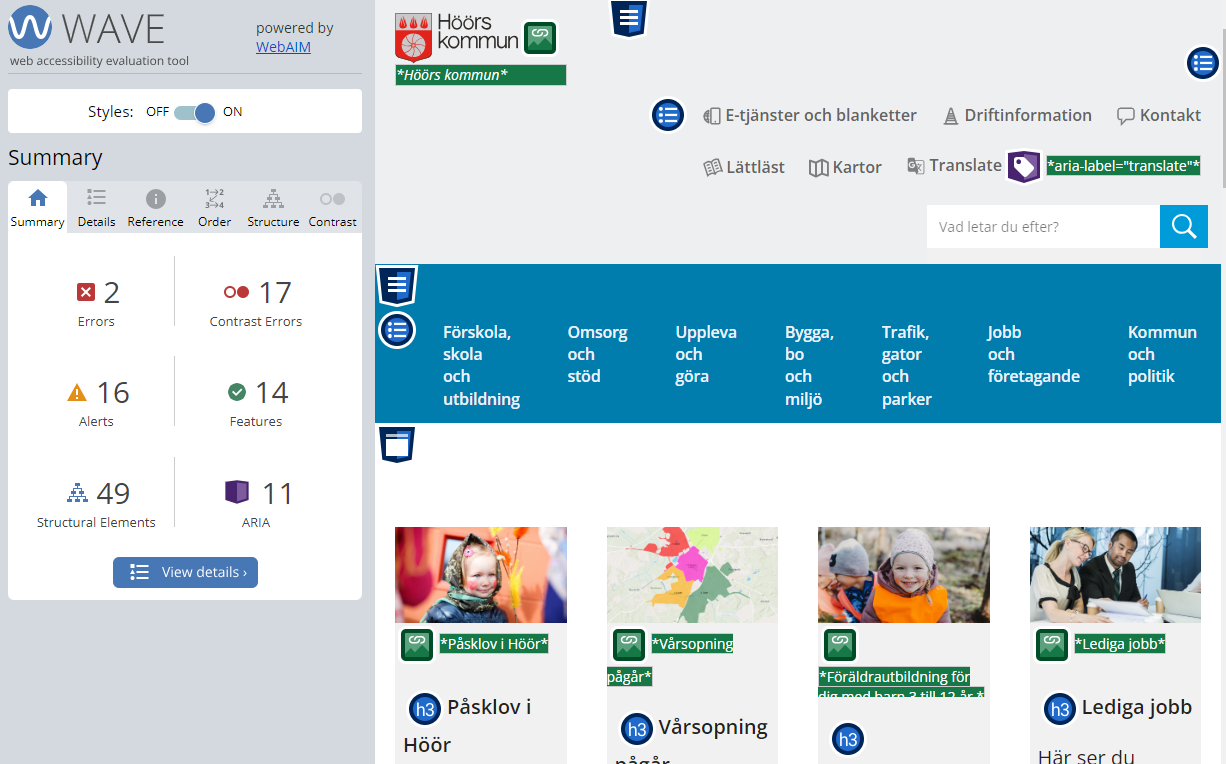
\includegraphics[width=1\textwidth]{../images/höörsKommunhemsida_WAVE.png} % Kanske skriva ett förklarande av bliden.
    WAVE resultatet från Höörs kommuns startsida.
    \end{center}
    I bilden finns själva webbsidan och en panel till vänster vilket är WAVE resultatet.
    Panelen innehåller:
    Erors, felaktiga html element eller felaktig användning av html element.
    Alerts, Potentiella problem med webbsidan.
    Structural element, hur många element som ger struktur på webbsidan som användes.
    De elementen har även ikoner som visas på webbsidan där de används.
    Contrast erors, kontrastfel.
    Features, tillägg som ökar användarvänligheten på webbsidan.
    Aria, hur många aria attribut som användes.
    Det finns även ikoner för vart aria användes på webbsidan.
    Under details går det att se en mer detaljerad beskrivning av allt i summary och läsa om de olika delarna.

    %I bilden kan man se att WAVE kontrollerar kontrasten på innehållet,redovisar HTML strukturen och vart ARIA används på webbplatsen.
    %Fell i HTML syntax redovisas enkelt och ikoner på webbsidan visas var olika element och attribut används.

    \subsubsection{Screen reader} %jens hade lite problem med det här men det kanske var okej som det var

    En screen reader är ett digitalt verktyg som läser upp textinnehåll i ett html element.
    Det finns WCAG krav där användaren programmässigt ska kunna bestämma vad något är och vad det har för funktion.
    Till exempel finns WCAG krav 1.3.5 Identify Input Purpose (Level AA) där användaren ska kunna programmässigt bestämma vilken information som ska skrivas in i ett textinmatningsfält.
    Med en screen reader ska den berätta för användaren att det är ett textinmatningsfält och vilken information som ska skrivas in.

    \subsection{Kommunala webbplatsern} % Är lite överallt.
    Kommuner har en webbplats där de lägger upp information om kommunen och hitta olika e-tjänster.
    Alla kommunala webbplatser ser inte lika dana ut och har olika funktionalitet.
    %Om man jämför webbplatser från olika kommuner ser man att utseendet och designen på webbplatserna är olika.
    På grund av att det finns en skillnad i utseendet finns det också en skillnad i hur webbplatsen är konstruerad och hur den är tillgänglighetsanpassad.
    Det finns också några kommuner med webbplatser som ser likadana ut bara att de har varierande innehåll.
    %För att meddela information om en kommun digitalt har kommuner hemsidor som det styr innehållet på och lägger upp information om kommunen.
    %Det som är intressant om kommunala hemsidor är att alla hemsidor inte ser likadan ut utan de flesta ser annorlunda ut.
    %Det finns också några kommuner med hemsidor som ser likadana ut bara att de har varierande innehåll.
    %Vissa kommuner har hemsidor som ser likadana ut bara varierande innehåll.
    %Skillnaden i hur kommunala hemsidor ser ut betyder att det finns en skillnad på hur de är uppbyggda och hur det är anpassade för användarvänlighet på webben.
    
    Webbsidorna i undersökningen valdes från en listan på \textcite{SverigesKommuner}.
    Listan är ordnad i folkmängd, störst till minst för alla kommuner i Sverige.
    För undersökningen valdes en webbplats som var bland de högst upp på listan, en i mitten av listen och en längst ner på listan.
    Kommunen som var högst upp på listan var \textcite{Linköpings_kommun}
    Kommunen i mitten av listan var \textcite{Höörs_kommun}
    Kommunen längst ner på listan var \textcite{Sorsele_kommun}
    %De valda kommunerna blev \textcite{Linköpings_kommun} (störst), \textcite{Höörs_kommun} (i mitten) och \textcite{Sorsele_kommun} (minst).
    
    \section{Metod och Material}

    Undersökningen utgick på att testa hur kommunernas webbplatser uppfyller alla krav i WCAG 2.2.
    Digg och W3C har givit ut en listor över hur kraven kan uppnås i lagen och WCAG 2.2.
    För specifikation om WCAG kraven se \textcite{WCAG_2.2}.
    Undersökningen utgick från en sammanställning över WCAG 2.2 kraven och hur de kan mötas.
    För att hitta den sammanställningen se bilaga 1.
    %Utifrån tabellen testades alla kraven på Webbplatserna.
    Nedan finns en förklaring av vad varje kolumn i kalkylarket består av.
    \begin{enumerate}
        \item Själva WCAG 2.2 kravet som skulle testas
        \item Hur WCAG 2.2 kravet ska testas
        \item På vilken webbplats som kravet testades
        \item Om webbplatsen uppfyllde kravet
        \item Kommentarer om webbplatsen
        \item På vilken webbplats som kravet testades
        \item Om webbplatsen uppfyllde kravet
        \item Kommentarer om webbplatsen
        \item På vilken webbplats som kravet testades
        \item Om webbplatsen uppfyllde kravet
        \item Kommentarer om webbplatsen
    \end{enumerate}

    \subsection{Ej testade krav}

    Det gjordes en avvikning från metoden för att 16 av WCAG 2.2 kraven inte kunde testas.
    På alla webbplatser så testades 70 vad de 86 WCAG 2.2 kraven.

    Det finns 3 krav som inte testades för att testaren inte var en del av de kommunerna.
    Krav 2.2.5 Re-authenticating (Level AAA) vilket handlar om att användaren loggar in igen efter att den har blivit utloggad utan dataförluster.
    \\ Krav 3.3.4 Error Prevention(Legal, Financial, Data) (Level AA) vilket handlar om förebyggande av fel vid finansiella transaktioner och lagligt bindande kontrakt.
    Till exempel att informationen ska kollas efter fel när användaren skriver in information för att köpa något.
    \\  Krav 3.3.6 Error Prevention (All) (Level AAA) vilket är typ samma som 3.3.4 fast det är inte endast för finansiella transaktioner och kontrakt.
    All information som användaren skickar in ska kollas efter fel och användaren ska kunna åtgärda de felen.

    11 av kraven inom synlighet kategorin testades inte.
    Kraven handlade om ljud och innehåller bland annat att det ska finnas undertexter och teckenspråkstolkning för videor och ljud.
    De testades inte av anledningen att ingen ljudfil eller videofil hittades på webbplatserna.

    Krav 2.1.4 Character Key Shortcuts (Level A) handlar om tangentbordsgenvägar och testades inte för att det inte fanns några tangentbordsgenvägar.

    Krav 2.2.4 Interruptions (Level AAA) handlar om att sidan uppdateras i nutid med ny information.
    Det kravet testades inte för att webbplatsen hade inga delar som uppdaterades i nutid.

    \section{Resultat} %Resultatet är fortfarande skrivet som skräp men det är lite svårt att göra på ett annat sätt.



    %Kanske bara borde sluta att vara lat och skriva en bra del till alla delar.
    %Kanske det lättaste är att bara ha en tabbel och sen utgå från den tabbelen.%
    \subsection{Synlighet krav}
    I den första delen av WCAG synlighet finns 29 krav varav 18 av de testades.
    Sorsele kommun mötte 10 och misslyckades med 8 av dem.
    Totalt lyckades kommunen med 55.56$\%$ av synlighet kraven.
    \\Höörs kommun mötte 13 och misslyckades med 5 av dem.
    Totalt lyckades kommunen med 72.22$\%$ av synlighet kraven.
    \\Linköpings kommun mötte 14 och misslyckades med 4 av dem.
    Totalt lyckades kommunen med 77.78$\%$ av synlighet kraven.
    \\I den här kategorin ligger Sorsele kommun klart lite bakom de andra kommunerna medans Linköping och Höörs kommun skiljer endast 1 krav.

    \newpage
    \begin{center}
    Synlighet (18 av 29 krav testades)

    \begin{tabular}{ |c|c|c|c|}
        \hline
        Kommun & Möter & Möter inte & Möter ($\%$) \\  \hline
        Sorsele & 10 & 8 & 55.64$\%$ \\ \hline
        Höör & 13 & 5 & 72.22$\%$ \\ \hline
        Linköping & 14 & 4 & 77.78$\%$ \\ \hline
    \end{tabular}
    \end{center}

    \subsection{Manövrerbar krav}
    I den andra delen av WCAG manövrerbar finns 34 krav varav 31 av de testades.
    Sorsele kommun mötte 21 och misslyckades med 10 av dem.
    Totalt lyckades kommunen med 67.74$\%$ av manövrerbar kraven.
    \\Höörs kommun mötte 30 och misslyckades med 1 av dem.
    Totalt lyckades kommunen med 96.77$\%$ av manövrerbar kraven.
    \\Linköpings kommun mötte 30 och misslyckades med 1 av dem.
    Totalt lyckades kommunen med 96.77$\%$ av manövrerbar kraven.
    \\Även i den här kategorin ligger Sorsele bakom men Linköping och Höörs kommun möte lika många krav.

    \begin{center}
    Manövrerbar (31 av 34 krav testades)

    \begin{tabular}{ |c|c|c|c|}
        \hline
        Kommun & Möter & Möter inte & Möter ($\%$) \\  \hline
        Sorsele & 21 & 10 & 67.74$\%$ \\ \hline
        Höör & 30 & 1 & 96.77$\%$ \\ \hline
        Linköping & 30 & 1 & 96.77$\%$ \\ \hline
    \end{tabular}
    \end{center}

    \subsection{Begriplighet krav}
    I den tredje delen av WCAG begriplighet finns 21 krav varav 19 av de testades.
    Sorsele kommun mötte 16 och misslyckades med 3 av dem.
    Totalt lyckades kommunen med 84.21$\%$ av begriplighets kraven.
    \\Höörs kommun mötte 18 och misslyckades med 1 av dem.
    Totalt lyckades kommunen med 94.73$\%$ av begriplighets kraven.
    \\Linköpings kommun mötte 18 och misslyckades med 1 av dem.
    Totalt lyckades kommunen med 94.73$\%$ av begriplighets kraven.
    \\Fortsatt är Linköpings kommun högst i antal möta krav med Höörs kommun rakt bakom och Sorsele kommun i sista plats

    \newpage
    \begin{center}
    Begriplighet (19 av 21 krav testades)

    \begin{tabular}{ |c|c|c|c|}
        \hline
        Kommun & Möter & Möter inte & Möter ($\%$) \\  \hline
        Sorsele & 16 & 3 & 84.21$\%$ \\ \hline
        Höör & 18 & 1 & 94.73$\%$ \\ \hline
        Linköping & 18 & 1 & 94.73$\%$ \\ \hline
    \end{tabular}
    \end{center}

    \subsection{Robust krav}
    Den fjärde och sista delen av WCAG är robust och där finns det bara 2 krav där båda testades.
    Sorsele kommun mötte 0 krav.
    Höörs kommun mötte 1 krav.
    Linköpings kommun mötte 1 krav.

    \begin{center}
    Robust (2 av 2 krav testades)

    \begin{tabular}{ |c|c|c|c|}
        \hline
        Kommun & Möter & Möter inte & Möter ($\%$) \\  \hline
        Sorsele & 0 & 2 & 0$\%$ \\ \hline
        Höör & 1 & 1 & 50$\%$ \\ \hline
        Linköping & 1 & 1 & 50$\%$ \\ \hline
    \end{tabular}
    \end{center}
    
    \subsection{Sammanfattning}
    Totalt lyckades Sorsele kommun möta 47 av kraven och misslyckades med 23 av dem vilket betyder att de mötte totalt 67.14$\%$ av kraven.
    Höörs kommun lyckades möta 62 av kraven och misslyckades med 8 av dem vilket betyder att de mötte totalt 87.14$\%$ av dem.
    Linköpings kommun lyckades möta 63 av de 70 kraven och mötte 90$\%$ av alla testade krav.

    \begin{center}
    Alla WCAG 2.2 krav (70 av 86 krav testades)

    \begin{tabular}{ |c|c|c|c|}
        \hline
        Kommun & Möter & Möter inte & Möter ($\%$) \\  \hline
        Sorsele & 47 & 23 & 67.14$\%$ \\ \hline
        Höör & 62 & 8 & 88,57$\%$ \\ \hline
        Linköping & 63 & 7 & 90$\%$ \\ \hline
    \end{tabular}
    \end{center}

    \section{Diskussion} %mer reflekterande, tänkande och tyckande
    Resultatet av Linköping kommun och Höörs kommun är väldigt lika.
    Det skiljer endast två krav mellan deras resultat.
    Linköping möter två krav som Höörs inte gör och Höörs ett krav som Linköpings inte möter.
    Det första kravet som  Höörs kommun misslyckas med är 1.1.1 Non-text Content (Level A), det ska finnas textalternativ till ej textbaserad media.
    Att bilder inte har bildtexter är förmodligen bara att personerna som underhåller webbsidan är för lata för att göra bildtexter eller inte förstår varför bildtext borde finnas.
    Det andra kravet är 1.4.11 Non-text Contrast (Level AA), kontrastfel.
    Kontrastproblemen är förmodligen bara att skaparna eller kommunen ville att designen skulle se ut på ett specifikt sätt.

    Kravet som Linköpings kommun inte möter är 1.3.5 Identify Input Purpose (Level AA), informationen som ska in i ett textfält ska kunna bestämmas med ett program.
    Linköpings kommun verkade hade samma inloggningssida som Sorsele kommun och det gick inte att programmässigt bestämma viken information som skulle in i textinmatningsfälten.
    Det är inte en så stor skillnad i antal möta krav som kanske skulle se likadan ut om andra kommuner valdes.
    %Jag tycker att det inte kan dras någon slutsats från den skillnaden utan jag skulle behöva testa mer webbplatser för att dra en slutsats.

    Den riktigt intressanta delen är Sorsele kommun som möter 15 mindre krav än Höörs kommun.
    Det är en drastisk skillnad jämfört med Höör och Linköping.
    Sorsele kommun klarar mindre krav i alla kategorier men det är mest i manövrerbar kategorin.
    Väldigt många av de misslyckande kraven relaterar till att användaren kan använda tab knappen på tangentbordet för att komma åt ett sökfält som inte visas.
    På Sorseles webbplats fanns det vissa funktioner bara på vissa delar av webbplatsen.
    Om man tryckte på länkar för att gå vidare försvann de funktionerna och hur webbsidan såg ut ändrades.
    Att navigera från till exempel ¨Omsorg och stöd¨ till ¨Orosanmälan för barn eller vuxen¨ ändrar helt sidans layout.
    Det var inte något som märktes på Linköpings eller Höörs kommun webbplatser.

    %Det här är väldigt subjektivt men känslan jag fick av Sorsele kommun var att den blev skapad och sen hade blivit uppdaterad ett flertal gånger av olika personer.
    %Att skapa en hemsida och sen uppdatera den flera gånger av olika företag med nya funktioner och efter nya regler kostar förmodligen mindre än att skapa en ny hemsida men hemsidan kommer förmodligen att behålla några av de dåliga delarna före uppdateringen.
    %Det är en kommun med liten befolkning så att uppdatera en sida är förmodligen mer logiskt med tanken på kommunens lägre inkomster än resten.
    %Jag fick inte den känslan av Linköpings eller Höörs kommun hemsida.

    För att resultatet ska visa något om kommuner generellt skulle fler kommuner undersökas.
    Den enda slutsatsen som kan dras är att det kanske finns en tendens till att kommuner med lägre antal invånare har en mindre användarvänlig hemsida.
    Att undersöka fler kommuner är också en väg att förbättra undersökningen och förstärka resultatet.
    Att testa fler kommuner på endast en del av WCAG 2.2 skulle förmodligen ge ett resultat där fler slutsatser skulle kunna dras.
    %Det går också att fördjupa sig mer i individuella WCAG krav och kontrollera dem mer noggrant.
    %\textcite{WCAG_2.2} innehåller för varje krav länkar med extra förklaring av innebörden av kravet och förslag på olika väga att testa krav.

    \newpage
    \section{Referenser}

    \printbibliography[heading=none]

    \newpage
    \section{Bilagor}
    Bilaga 1
    Google spreadsheet:
    \\ https://docs.google.com/spreadsheets/d/e/
    \\2PACX-1vT4b-RPc7sfET2uvwcBs0txumqoLYv5NLsBbLu82YSxWc5ZTy
    \\\_H3eZAPPYyOzse4R0AE8LfQ24HFca-/pubhtml

    Google spreadsheet som pdf:
    \\https://github.com/Mephit299/Gymnasiearbete/blob/master/Metod-Resultat.pdf

    \end{otherlanguage}
\end{document}
